%csky stuff
\chapter{Time-Integrated Search}

This chapter describes the time-integrated stacking search, starting with the properties of the analysis, followed by a description of the background trials and finally the signal trials with the result of the sensitivity and the discovery potential.
The search covers different spectral indices for the signal event emission.

\section{Analysis properties}

This section shows some of the underlying PDFs csky uses to calculate the test statistic values.
Since csky is based on PDF ratios for practical reasons, not all individual PDFs can be shown clearly.
Consequently, here are a few basic PDFs and ratios whose form is apriori important for the quality of the analysis.

\subsection{Background space PDF}

The background space PDF is generated with data and only depends on the declination $\delta$ of the events, given by the almost right ascension symmetry of the IceCube detector due to its position.
It is normalized over the whole sky, hence satisfying the condition
\begin{align}
  \int d\Omega f = \int d\alpha \int d(\sin(\delta)) f = 1
\end{align}
and is shown in figure \ref{fig:bg_param_time_int}.
Lastly a spline, interpolating between the bin centers, is used to evaluate the events.
\begin{figure}
    \centering
    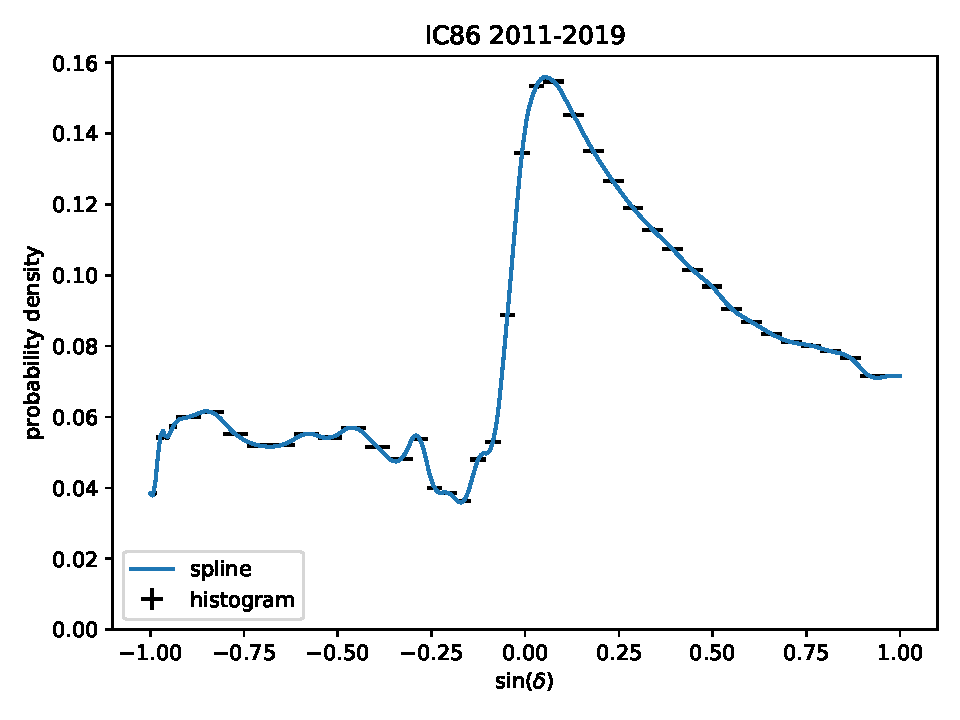
\includegraphics[width=\linewidth]{Plots/05_csky/bg_space_pdf.pdf}
    \caption{Background space PDF used in this analysis in $\sin{(\delta)}$ for all $\num{9}$ years, 2011-2019.}
    \label{fig:bg_param_time_int}
\end{figure}
The background space parametrization results in one plot only because all datasets underwent the same data processing pipeline.
The PDF shows a lower contribution for downgoing events and a higher one for upgoing events coming from the sides.
This result is compatible with other analyses, for example ...

\subsection{Energy ratio PDF}

The energy PDF ratios for different spectral indices $\gamma$ can be seen in figure \ref{fig:energy_ratio_time_int}.

\begin{figure}
    \centering
    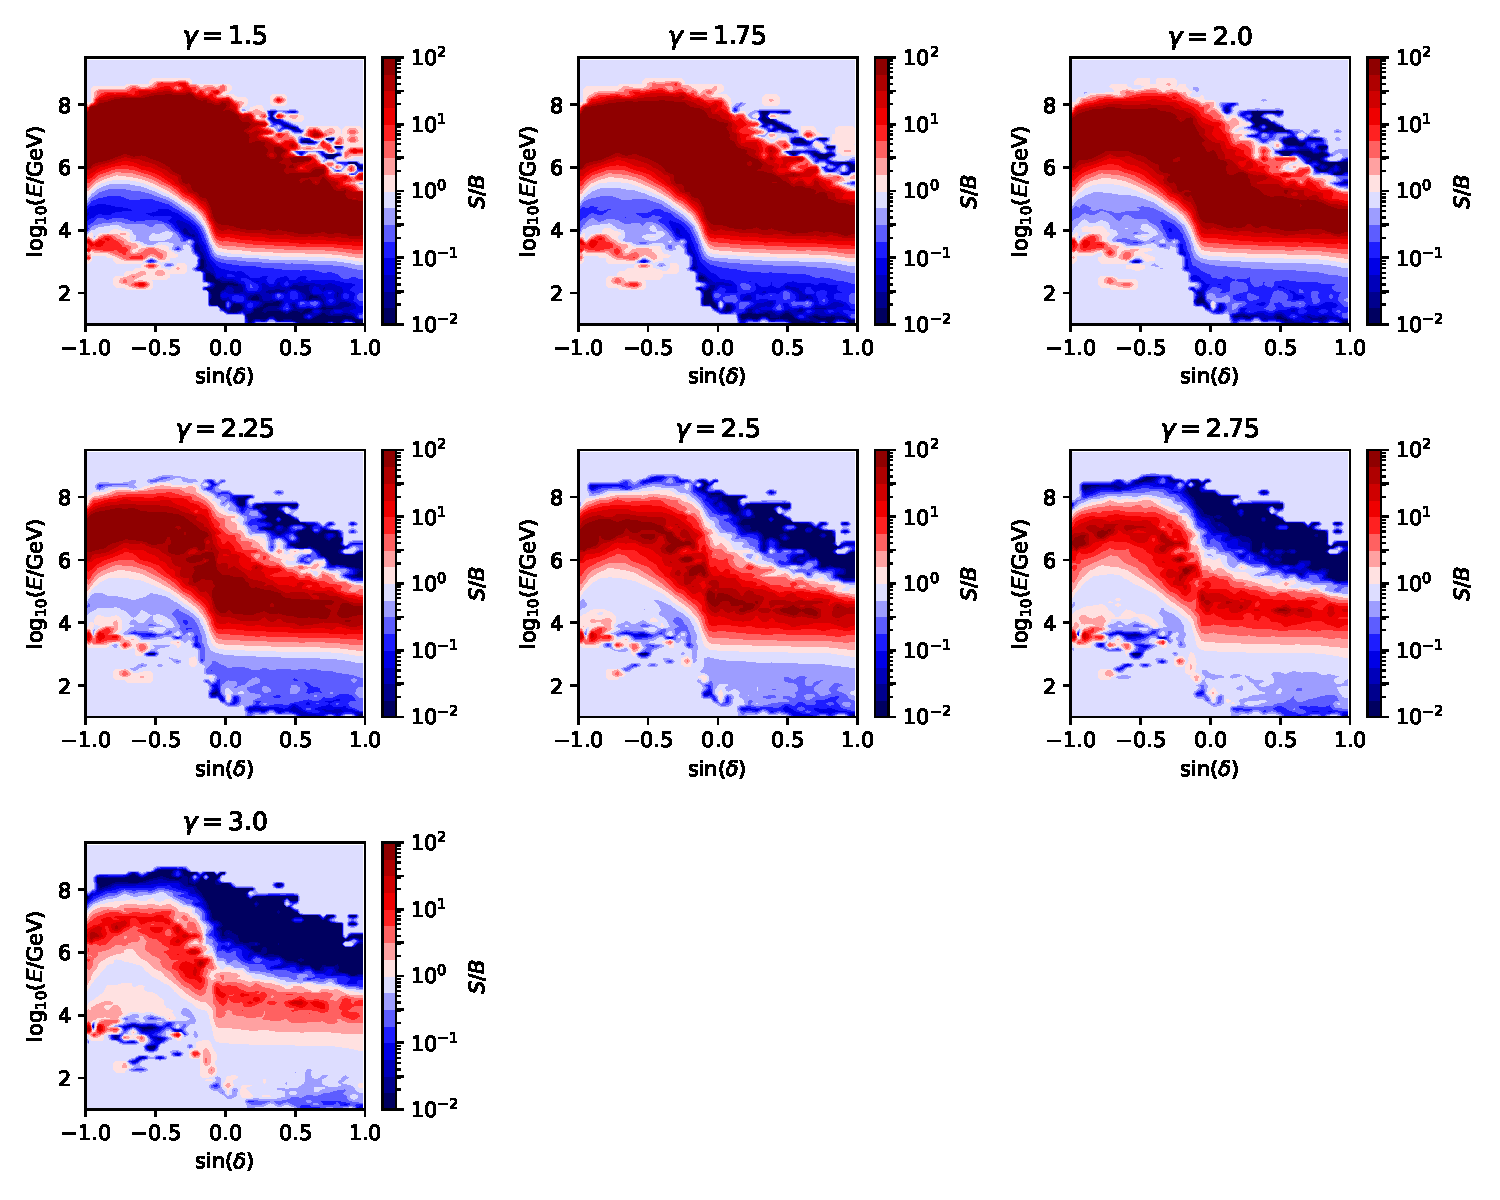
\includegraphics[width=\linewidth]{Plots/05_csky/energy_pdf_ratio.pdf}
    \caption{Energy PDF ratios used in this analysis in $\sin{(\delta)}$ and $\sin{\log{(E)}}$ for all $\num{9}$ years, 2011-2019, for different spectral indices $\gamma$.}
    \label{fig:energy_ratio_time_int}
\end{figure}

Mention high values in upper right (okay since they bias towards lower sens values (weaken)) and lower left (bad, bias towards higher sens values)

\section{Background Trials}

mention stacking

The histogram of the background test statistic values can be seen in figure \ref{fig:bg_ts_time_int}.
The number of trials processed is $\num{974000}$\footnote{Originally $\num{e6}$, but some jobs fail due to various technical reasons.}.
Important features of the plot are that the $\chi^2$ distribution has as straight a tail as possible.
This is reflected in the number of degrees of freedom $dof$ in the $\chi^2$ distribution.
This should be as close to 1 as possible, which corresponds to a pure background statistic without signal.
The test statistic should also be symmetrical around the zero point.
A shift around the zero point is an indication of an undesired bias of the statistic.
Therefore, the value of the quotient of the number of positive and negative events should ideally be $\eta = \num{0.5}$.
Apart from the fit parameters, the median and $5\sigma$ deviation value of the test statistic are necessary for the subsequent calculation of the sensitivity and the discovery potential.

The fit parameters of the background test statistic are
\begin{align}
  dof &= \num{1.115},\\
  \eta &= \num{0.656}
\end{align}
and the key values later to be processed are as follows\footnote{Some analyses use the $3\sigma$ value for the discovery potential.}
\begin{align}
  median &= \num{0.140},\\
  3\sigma &= \num{10.651},\\
  5\sigma &= \num{28.060}.
\end{align}

\begin{figure}
    \centering
    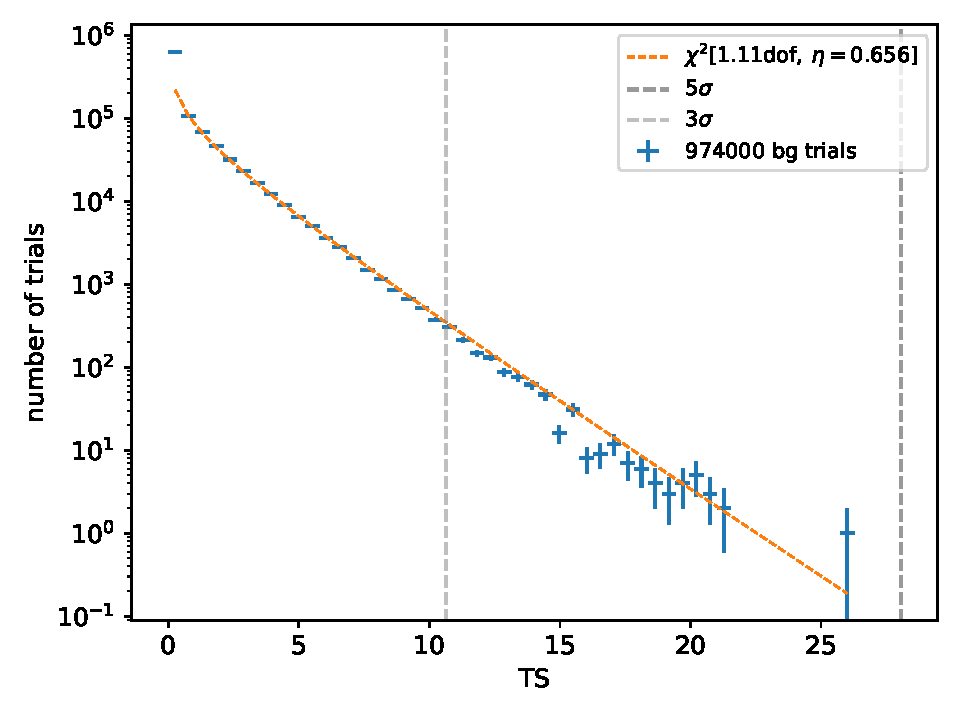
\includegraphics[width=\linewidth]{Plots/05_csky/9_years_gfu_gold_bg_new.pdf}
    \caption{Histogram of the background test statistic for the time integrated analysis. Shown are also the number of degrees of freedom $dof$ and the ratio of positive and negative values $\eta$.}
    \label{fig:bg_ts_time_int}
\end{figure}

\section{Signal Trials}

Before calculating the sensitivities and discovery potentials, certain properties of the likelihood or its behaviour should be investigated.
Since the spectral index $\gamma$ and the signal parameter $n_\text{S}$ are fitted, it is advisable to look at the likelihood environment to check for a smooth landscape to ensure a fit is possible and to exclude any other unwanted local maxima.
A scan of the parameter space for one likelihood can be seen in figure \ref{fig:llh_scan_time_int}.
Although there is a relatively flat maximum, the likelihood environment does not show any strange behaviour.
\begin{figure}
    \centering
    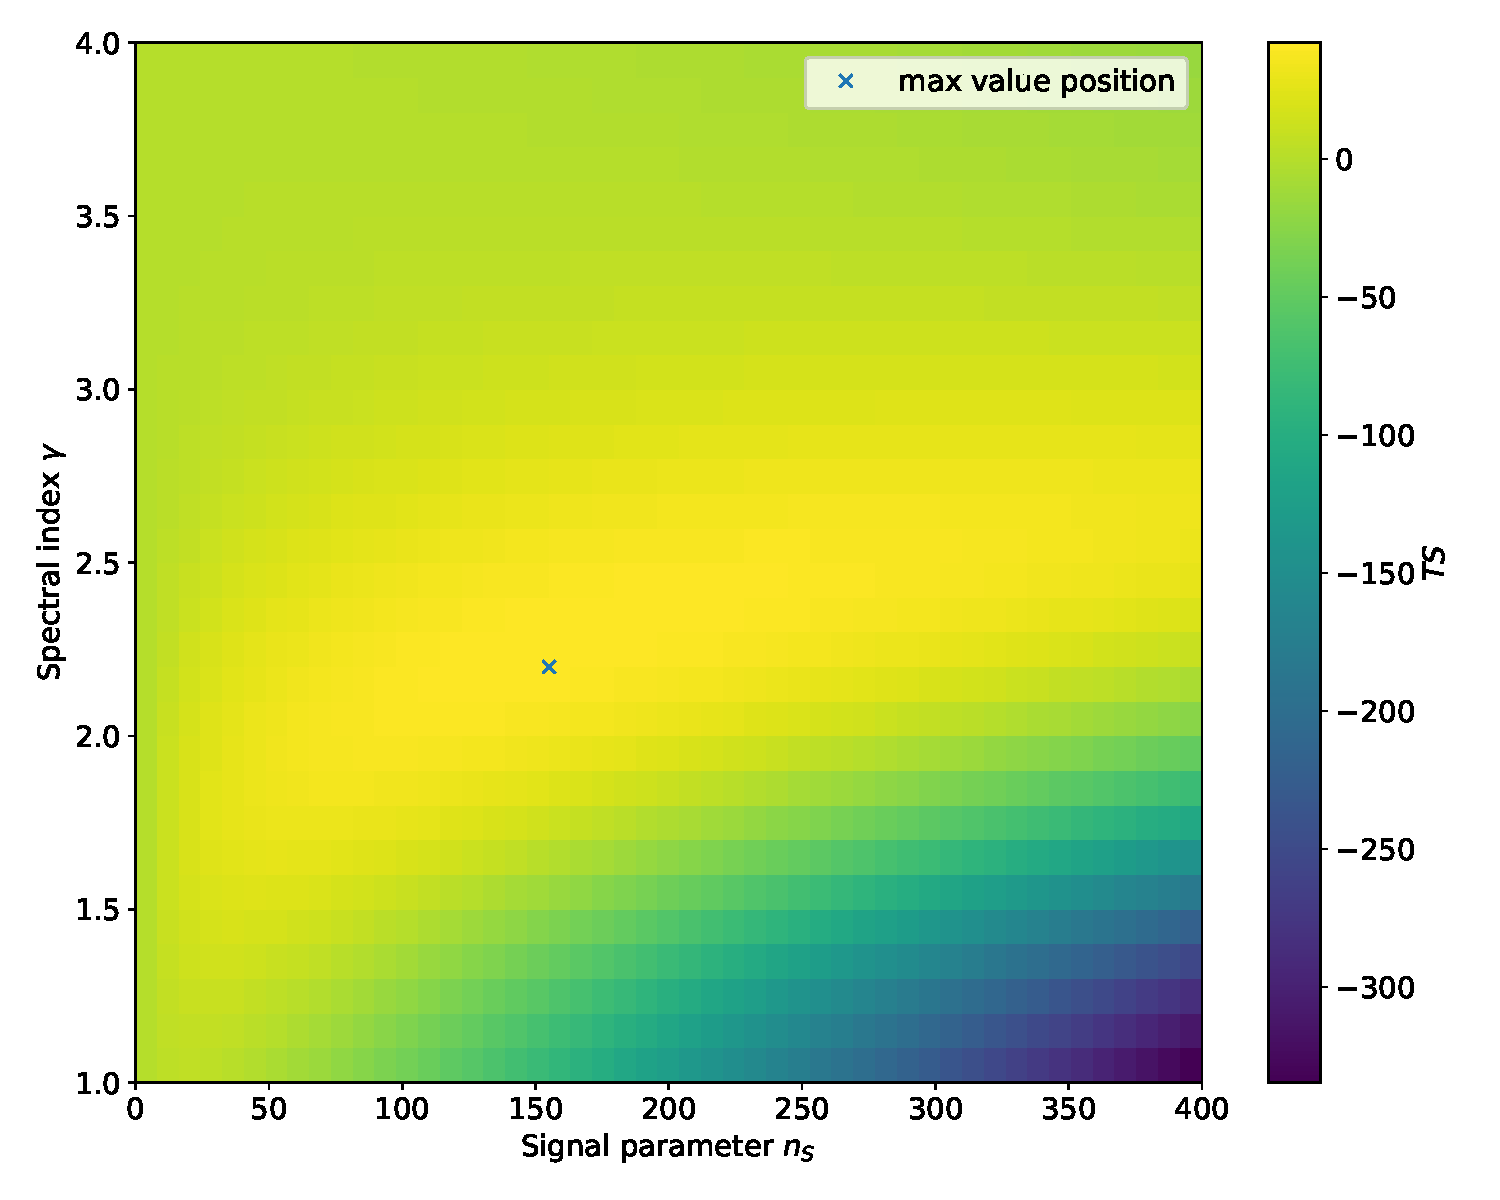
\includegraphics[width=\linewidth]{Plots/05_csky/llh_scan_time_int.pdf}
    \caption{Scan of one likelihoodspace for the time integrated analysis in the spectral index $\gamma$ and the signal parameter $n_\text{S}$. The number of induced signal events is $n_S = \num{100}$ with a spectral index of $\gamma = 2$. The maximum test statistic value is marked in the plot including the contours of $\num{1}\sigma$ and $\num{2}\sigma$.}
    \label{fig:llh_scan_time_int}
\end{figure}
The method of the calculation of the contours comes from \cite{Blobel} and corresponds to the maximum of the negative log-likelihood after subtracting $\num{0.5}$ and $\num{2}$ accordingly to get the $1\sigma$ and $2\sigma$ range, respectively.

After the fit behaviour has been checked, the signal can be injected.
With a higher number of signal events, the test statistic shifts to higher values, eventually reaching the thresholds set for the sensitivity and discovery potential.
Practically csky provides methods to apriori get an estimation of the number of signal events that have to be injected to satisfy certain thresholds without having to run a lot of trials on a cluster first.
The determined list of the number of signal events injected for the trials can be seen in table \ref{tab:signal_injected}.
The resulting CDFs for the time integrated sensitivities and discovery potentials can be seen in figure \ref{fig:cdf_sens} and \ref{fig:cdf_disc}.
Each point corresponds to the percentage of the test statistic being passed the thresholds mentioned in chapter \ref{sec:theory}.
\begin{figure}
    \centering
    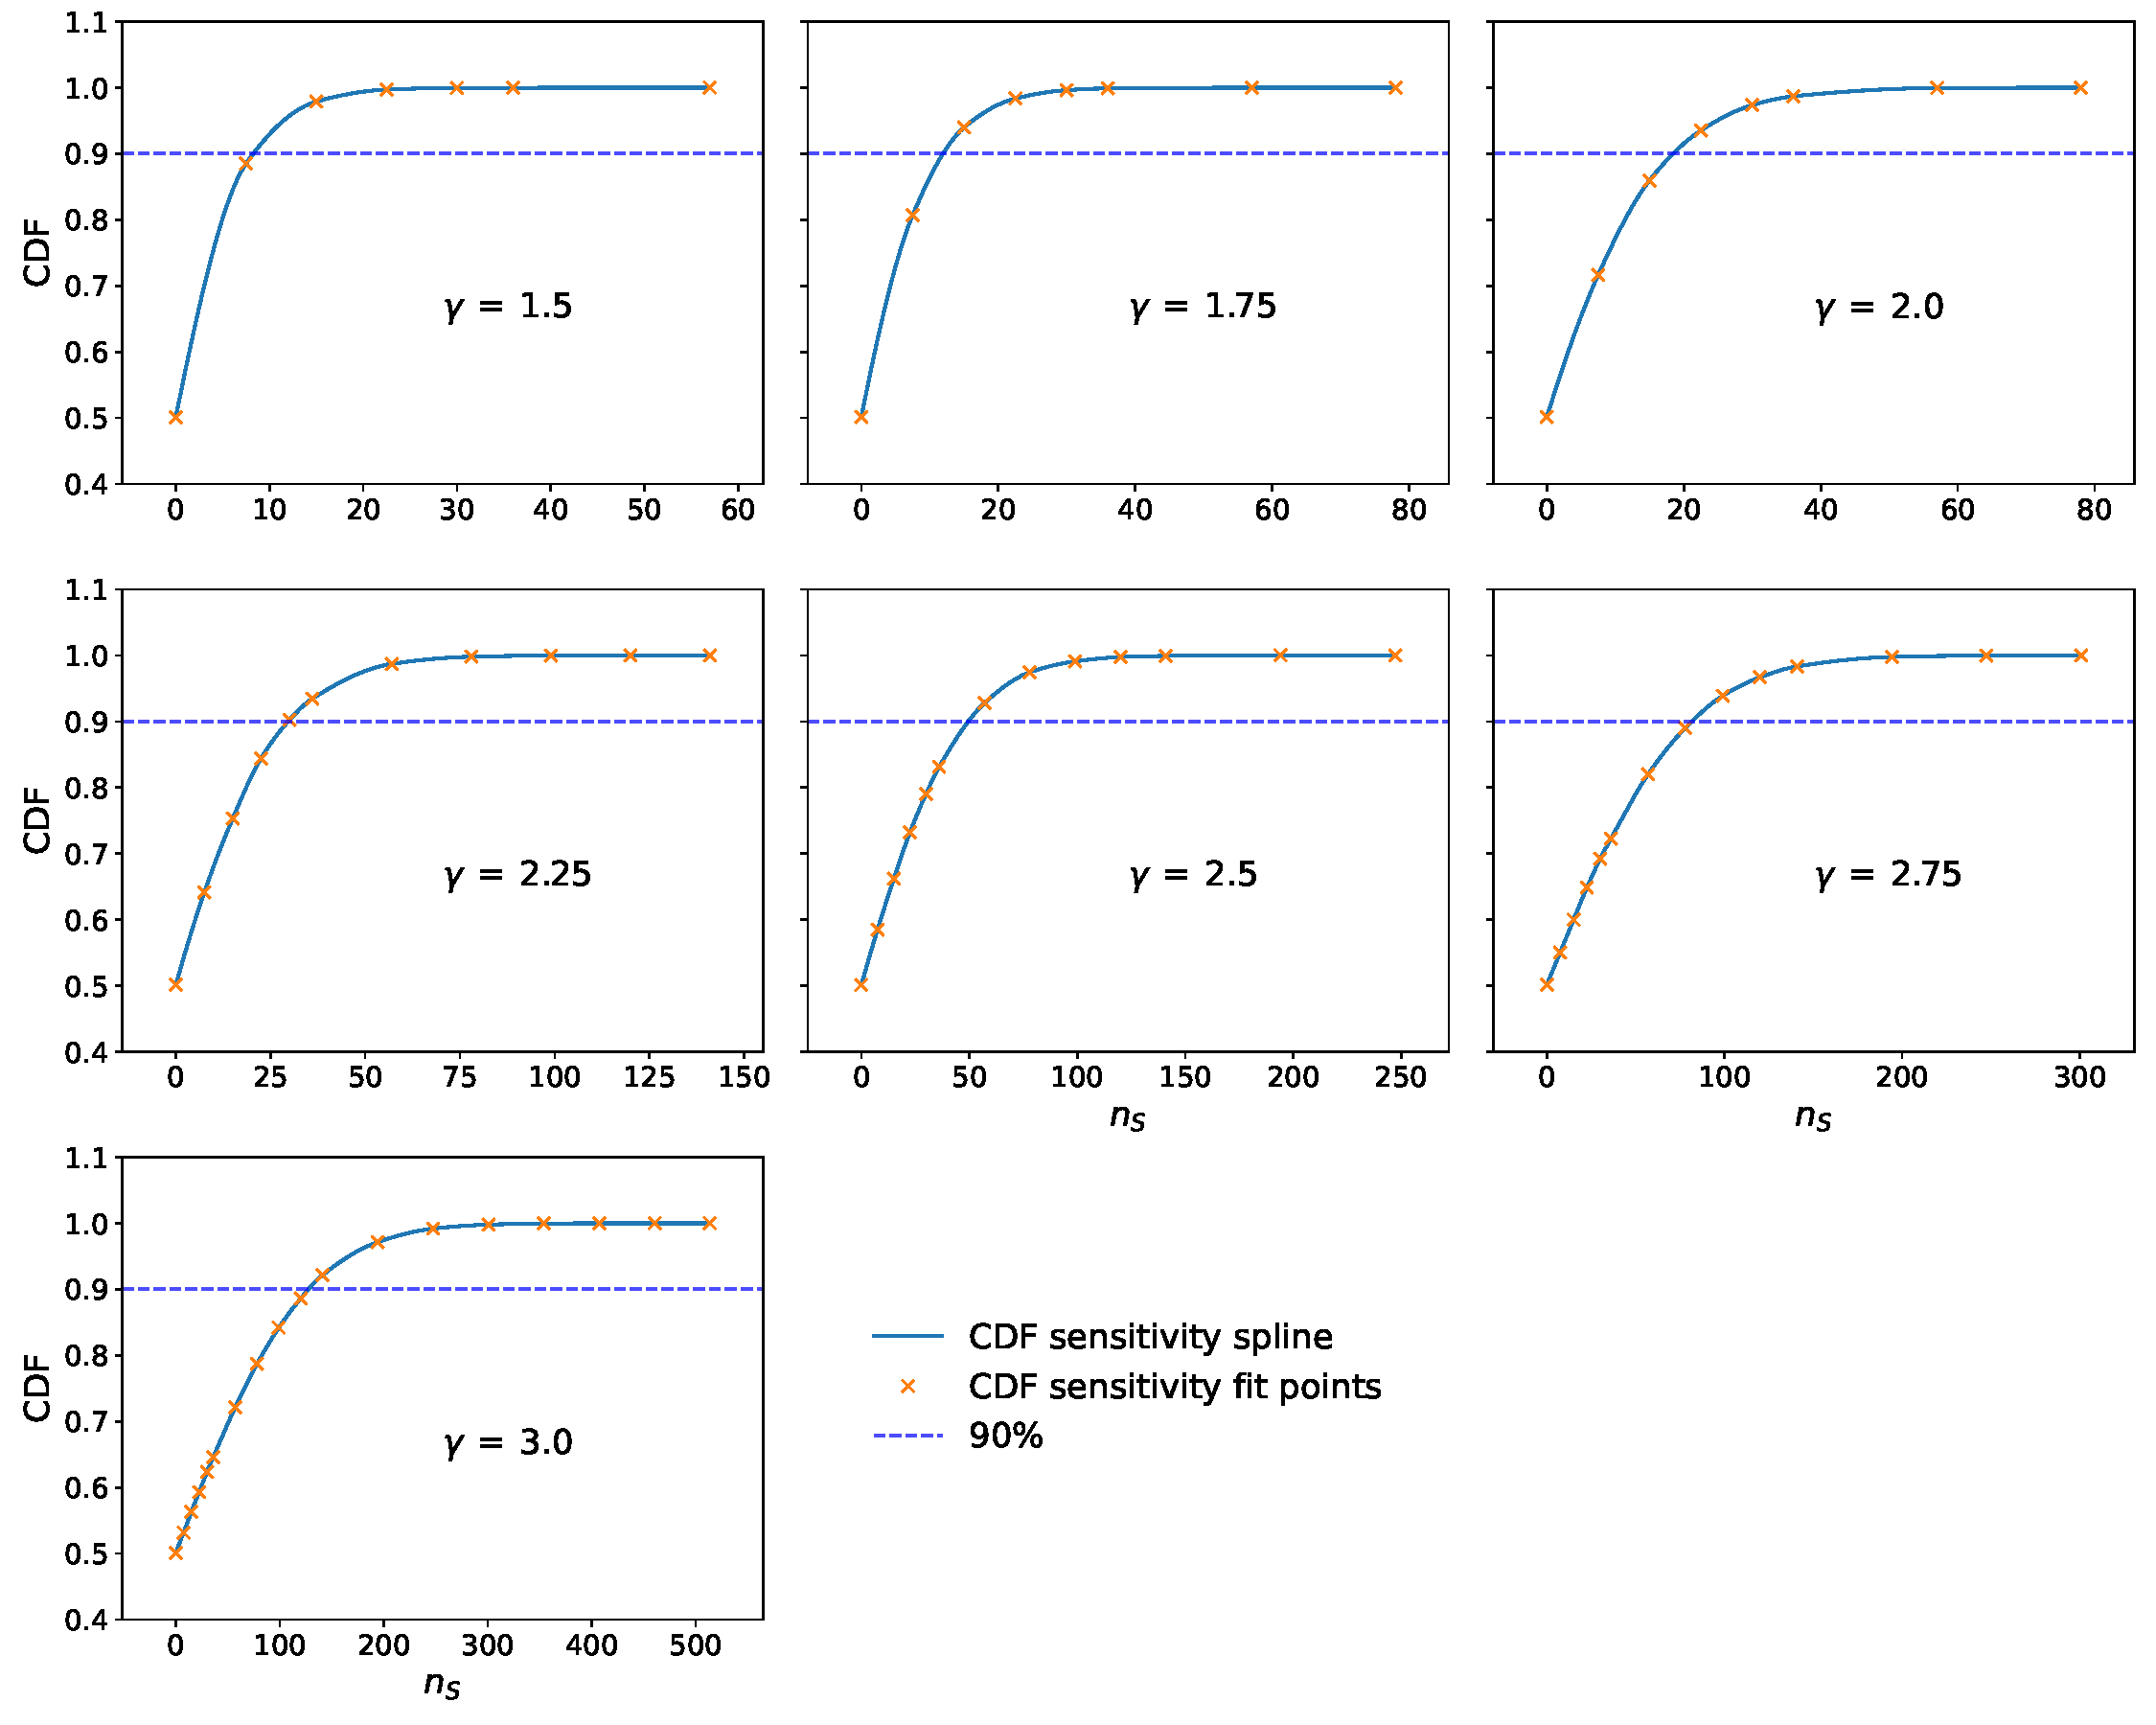
\includegraphics[width=\linewidth]{Plots/05_csky/9_years_gfu_gold_cdf_sens.pdf}
    \caption{Quantiles of the signal trials for the calculation of the sensitivity for the time integrated analysis at different spectral indices $\gamma$. A $\chi^2$ CDF fit provides a more accurate estimate of the sought signal parameter $n_\text{S}$ which satisfies the sensitivity condition at $\SI{90}{\percent}$.}
    \label{fig:cdf_sens}
\end{figure}
Note that all plots in figure \ref{fig:cdf_sens} start at about $\SI{50}{\percent}$ with a signal parameter of $n_\text{S} = 0$.
Since the absence of a signal parameter produces the background test statistic, the statistics share the same median, hence there will always be $\SI{50}{\percent}$ of the signal test statistic above the median of the background test statistic.
\begin{figure}
    \centering
    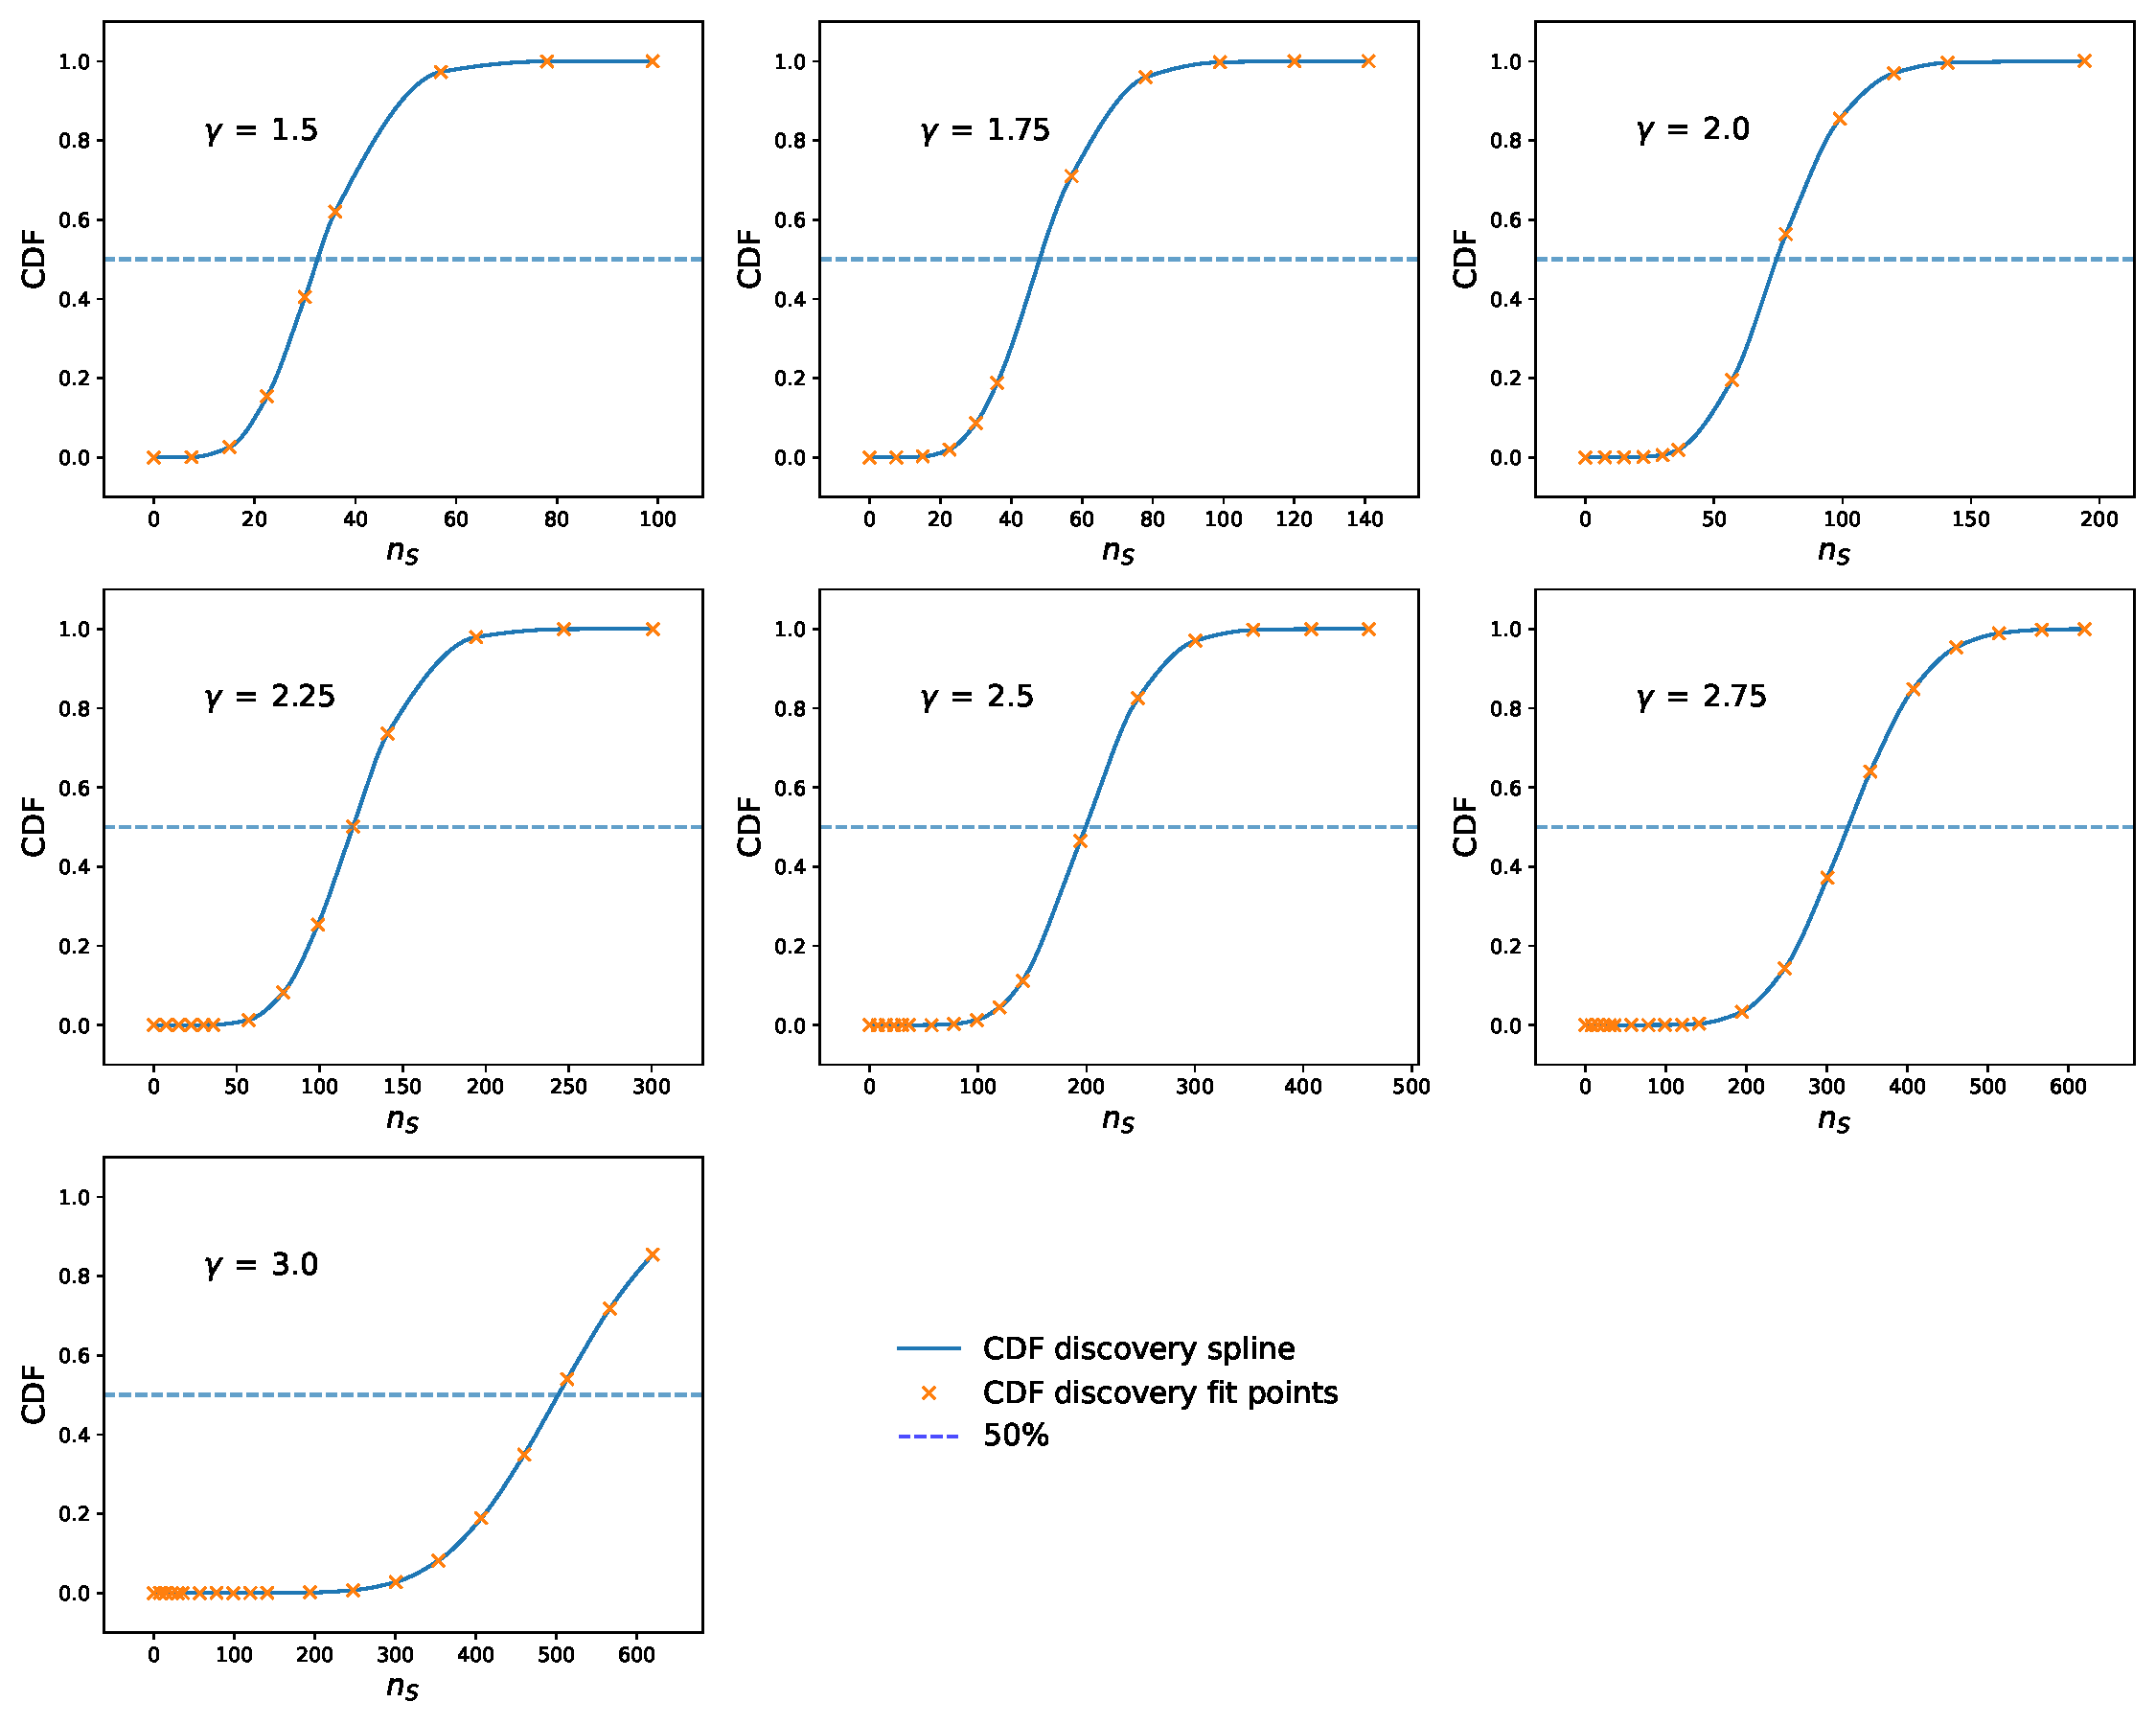
\includegraphics[width=\linewidth]{Plots/05_csky/9_years_gfu_gold_cdf_disc.pdf}
    \caption{Quantiles of the signal trials for the calculation of the discovery potential for the time integrated analysis at different spectral indices $\gamma$. A $\chi^2$ CDF fit provides a more accurate estimate of the sought signal parameter $n_\text{S}$ which satisfies the condition of the discovery potential at $\SI{50}{\percent}$.}
    \label{fig:cdf_disc}
\end{figure}
The sensitivities and discovery potentials from the CDFs can be seen in figure \ref{fig:sens_disc_time_int} and additionally in table \ref{tab:sens_disc_time_int}.
The values rise for higher spectral indices since the signal looks more background like the closer the spectral index is to $\gamma = 3$.
\begin{figure}
    \centering
    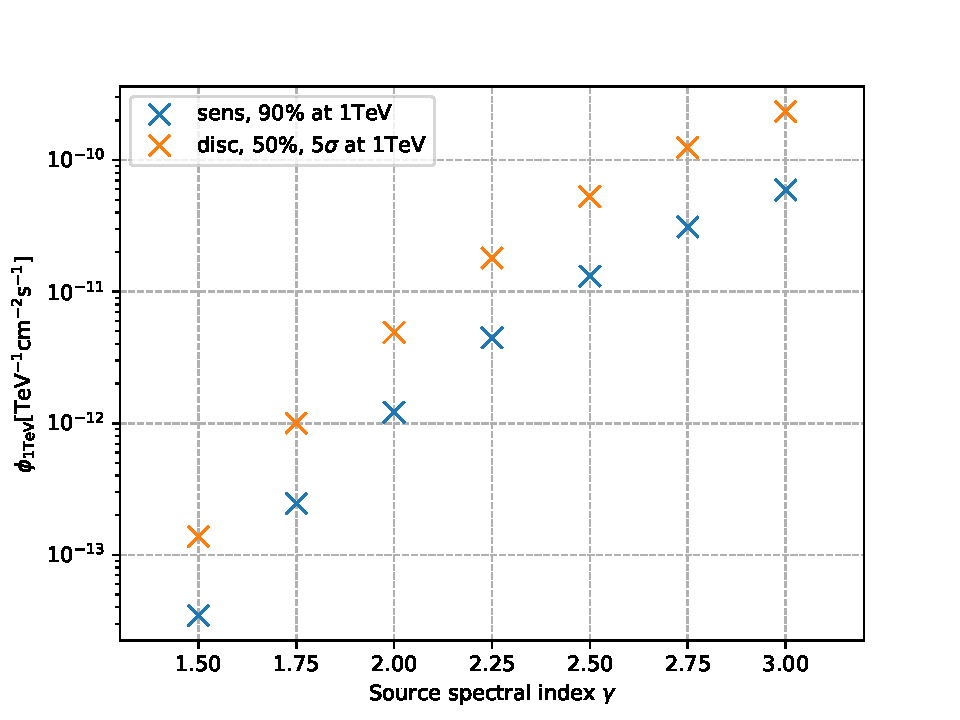
\includegraphics[width=\linewidth]{Plots/05_csky/time_int_sens_gfu_gold_9_years_new.pdf}
    \caption{Sensitivities and discovery potentials of the time integrated analysis for different spectral indices $\gamma$. The reference energy is $E_0 = \SI{1}{\tera\electronvolt}$.}
    \label{fig:sens_disc_time_int}
\end{figure}

\begin{table}
  \centering
  \caption{Sensitivities and discovery potentials for different spectral indices $\gamma$ at a reference energy of $E_0 = \SI{1}{\tera\electronvolt}$ for the time integrated analysis. Additionally the fitted number of signal events $N_\text{sig}$ satisfying the thresholds is shown.}
  \begin{tabular}{crcrc}
    \toprule
    $\gamma$ & $N_\text{sig,sens}$ &  sens in $\si{\tera\electronvolt\tothe{-1}\centi\meter\tothe{-2}\second\tothe{-1}}$ & $N_\text{sig,disc}$ & disc in $\si{\tera\electronvolt\tothe{-1}\centi\meter\tothe{-2}\second\tothe{-1}}$ \\
    \toprule
      1.50 & 8.16 & \num{3.45e-14} & 32.54 & \num{1.38e-13} \\ 1.75 & 11.86 & \num{2.46e-13} & 48.31 & \num{1.00e-12} \\ 2.00 & 18.39 & \num{1.21e-12} & 74.47 & \num{4.90e-12} \\ 2.25 & 29.65 & \num{4.46e-12} & 119.72 & \num{1.80e-11} \\ 2.50 & 49.21 & \num{1.31e-11} & 198.59 & \num{5.28e-11} \\ 2.75 & 81.12 & \num{3.10e-11} & 325.80 & \num{1.25e-10} \\ 3.00 & 127.62 & \num{5.93e-11} & 502.13 & \num{2.33e-10} \\ 
    \toprule
    \label{tab:sens_disc_time_int}
  \end{tabular}
\end{table}

\section{Examination of Fit Bias}

Several crosschecks can be made to examine the quality of the analysis results.
One of them is to check the fit of the parameters $\gamma$ and $n_\text{S}$ for bias.
The fit behaviour of the analysis can be seen in figure \ref{fig:fit_bias_gamma} for $\gamma$ and in figure \ref{fig:fit_bias_ns} for $n_\text{S}$.
The fitted spectral index is generally larger than the injected one and starts of at a spectral index of around $\hat\gamma = \num{3}$ with no injected signal events, because no signal events are equivalent to the statement that only background exists which has a spectral index of $\gamma = \num{3}$.
The larger fitted spectral index makes the analysis more conservative and therefore is not harmful for the overall results at spectral indices up to $\gamma = \num{2.5}$.
For higher spectral indices the fitted $\hat\gamma$ starts to sink below the set spectral index, since it is hard to fit for signal events that look like background. On the contrary this is harmful to the analysis results.
Equivalent behaviour can be seen for the fitted signal parameter $\hat{n}_\text{S}$.
\begin{figure}
    \centering
    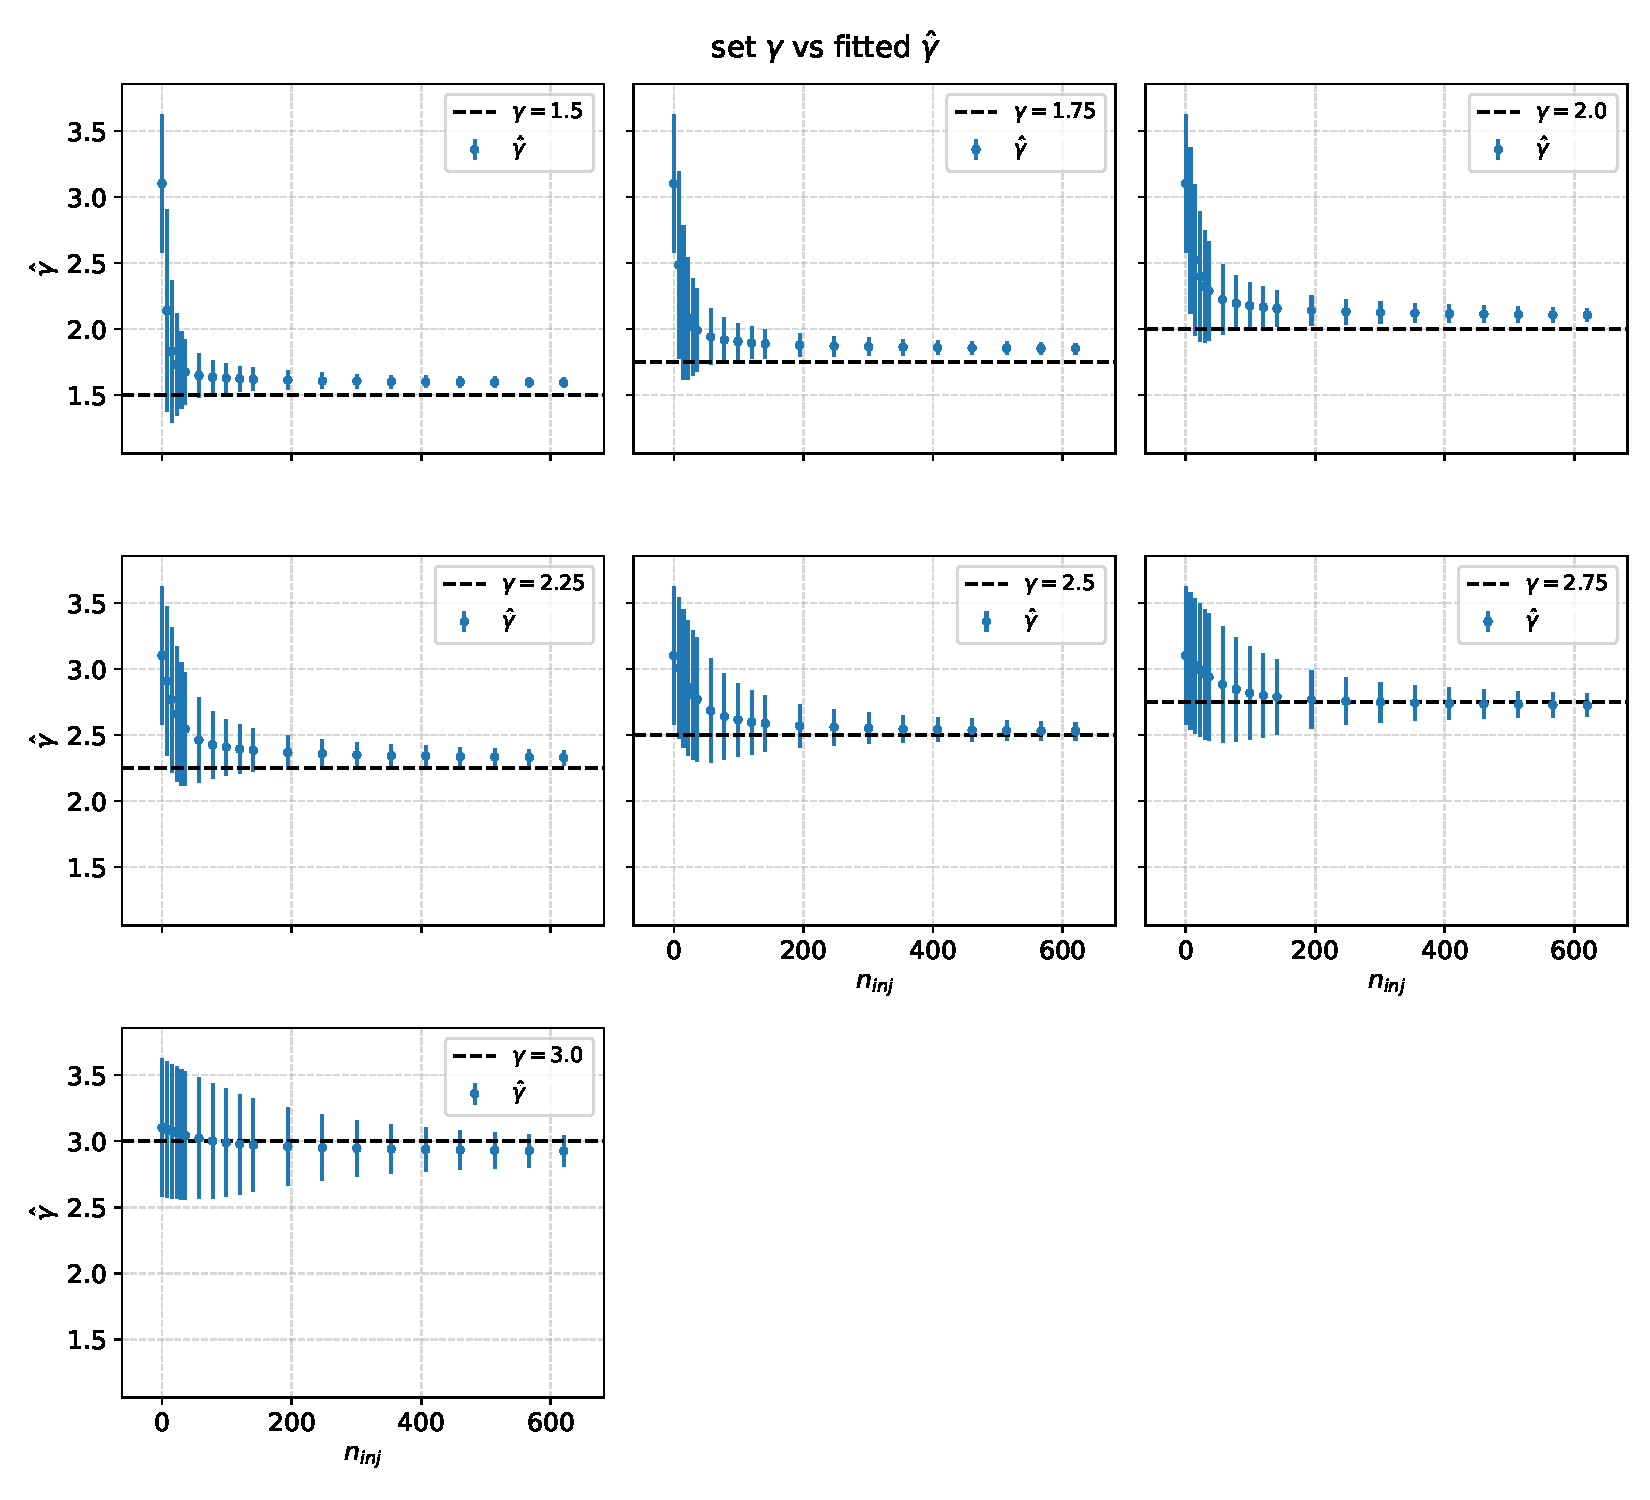
\includegraphics[width=\linewidth]{Plots/05_csky/gamma_fit_auto_3.pdf}
    \caption{Fitted spectral index $\hat\gamma$ in dependence of the injected number of signal events $n_\text{inj}$ with spectral index $\gamma$, shown with a horizontal black dashed line, for the trials used in the time integrated analysis.}
    \label{fig:fit_bias_gamma}
\end{figure}

\begin{figure}
    \centering
    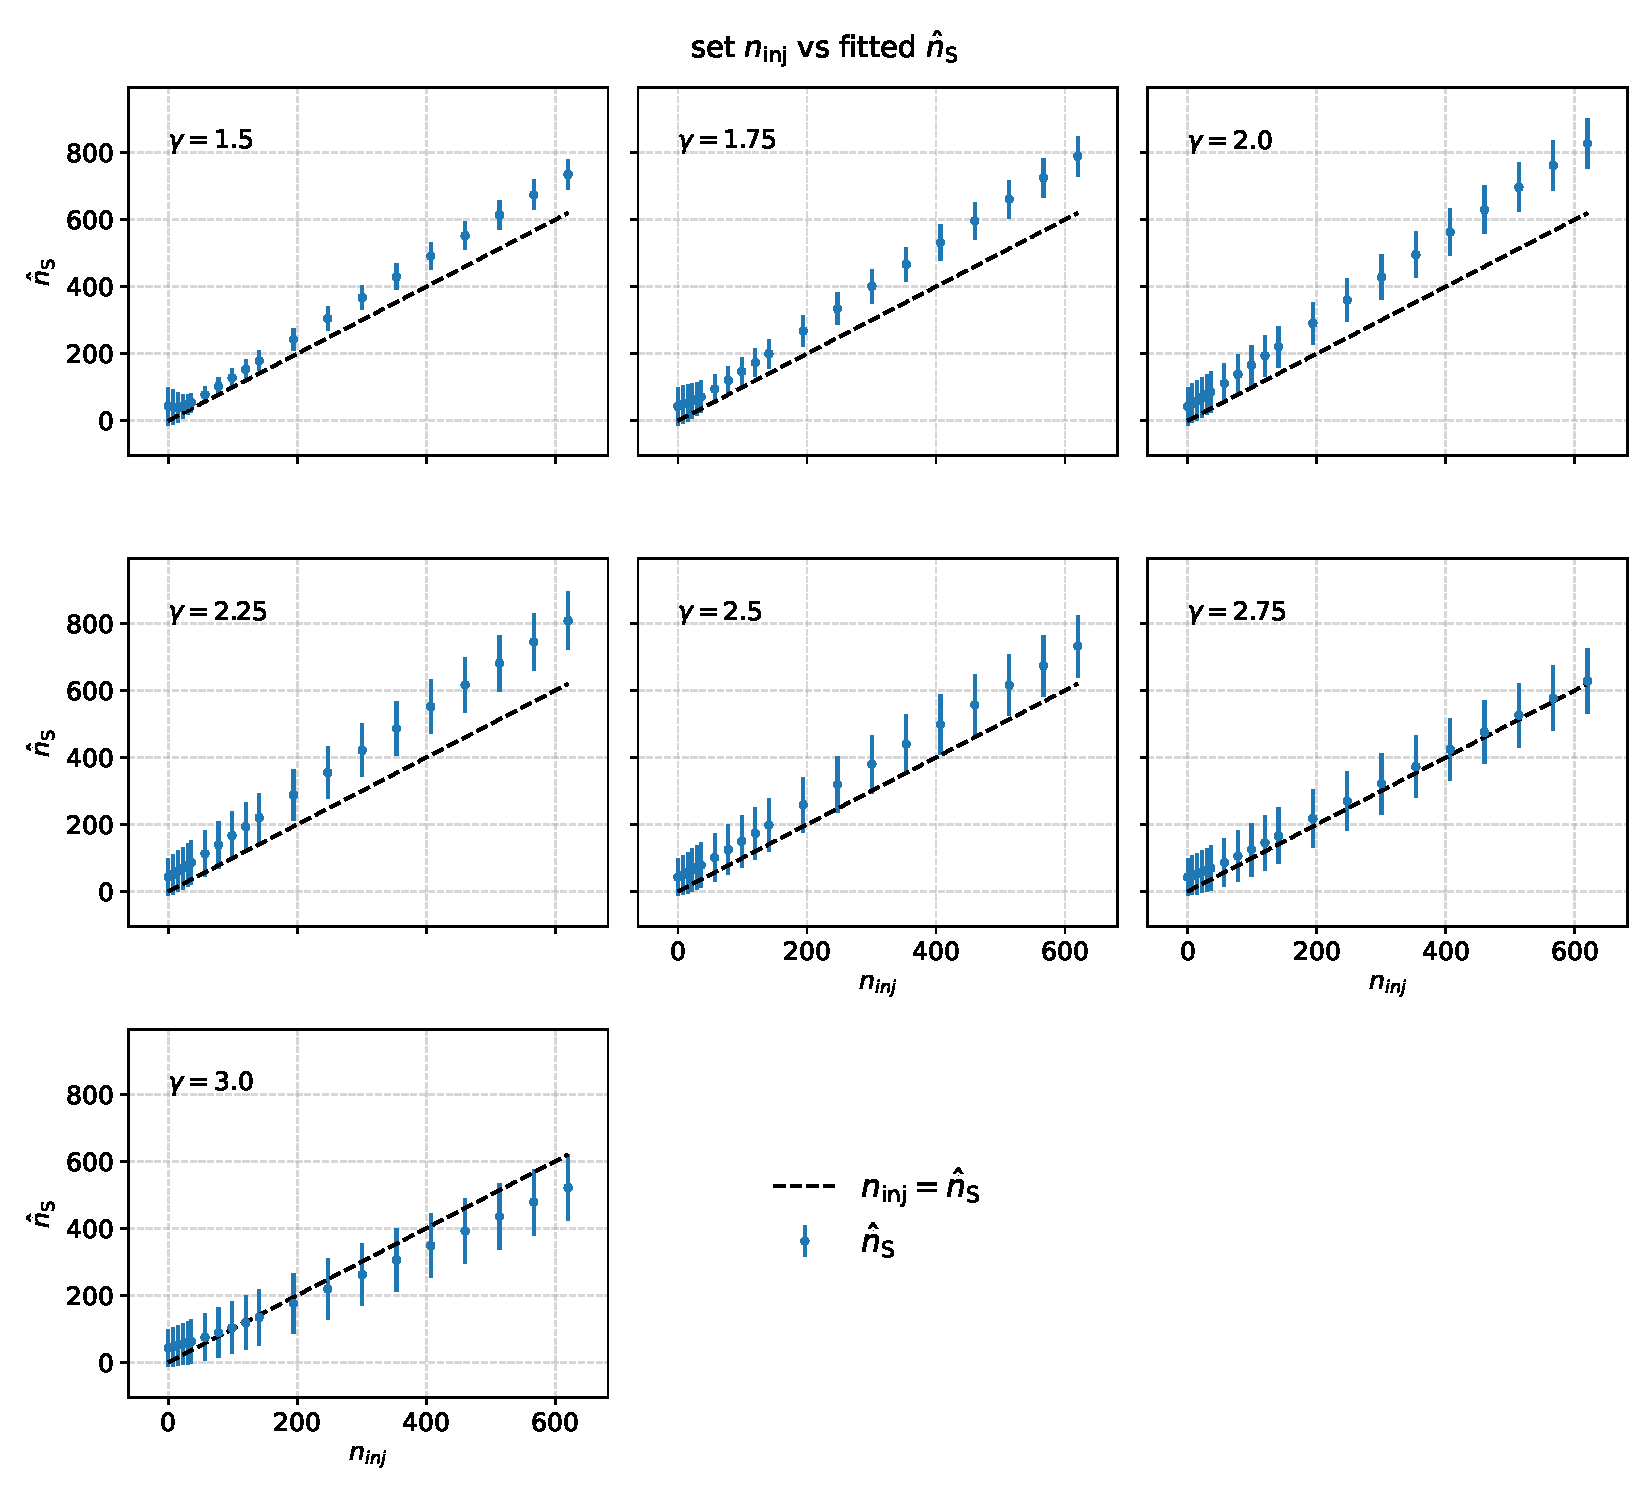
\includegraphics[width=\linewidth]{Plots/05_csky/ns_fit_auto_4.pdf}
    \caption{Fitted number of signal events $\hat{n}_{\text{S}}$ in dependence of the injected number of signal events $n_\text{inj}$ with spectral index $\gamma$ for the time integrated analysis. The black dashed line shows the equality of fitted and injected number of signal events.}
    \label{fig:fit_bias_ns}
\end{figure}

\chapter{Time-Dependent Search} \label{sec:csky_time_dep}

The time-dependent search examines $\num{10}$ sources independently of each other.
Ideally, all gfu-gold alerts should be examined and, in addition, preferably stacked.
However, time-dependent stacking is not yet sufficiently implemented in csky during the development of this thesis, and examining all sources individually would require too much computing capacity.
Chapter \ref{sec:tdepps} contains more detailed information on the technical details of time-dependent stacking.
Therefore, only the $\num{10}$ alerts with the highest signalness in the set are used as sources.
These can be seen in table \ref{tab:sources_time_dep}.

This analysis uses an untriggered flare procedure in which the temporal centre of the flare $t_0$ is set to the time of the source while the length $dt$ of the flare in shape of a box is fitted.
The time window is qualitatively expanded between two events at which the test statistic is maximised.
The maximum length of the time window is allowed to be $\SI{200}{\day}$.
This conservative approach results from the fact that no assumptions are made about the temporal emission behaviour of the source.
The maximum length of the time window of $\SI{200}{\day}$ is based on the $\SI{158}{\day}$ time window of the txs analysis \cite{txs}.

The figures shown for this analysis refer to source number $\num{11}$ and the figures for all sources are shown in the appendix in chapter \ref{sec:time_dep_search_appendix}, as the plots of all sources are quite similar and thus a better representation is ensured.

\section{Background Trials}

The background trials for source number $\num{11}$ are shown in figure \ref{fig:bg_trials_time_dep_1} and additionally for all $\num{10}$ sources in figure \ref{fig:bg_trials_time_dep} in the appendix.
Since the length $dt$ of the time windows is fitted, the number of degrees of freedom is generally greater than in the time integrated analysis.
The $\chi^2$ distribution generated via the trials is thus somewhat more convex.
The values to calculate the fluences can be seen in table \ref{tab:sigma_time_dep}.
In addition to the test statistics values, the time windows of the background trials can be examined.
These are shown in figure \ref{fig:bg_trials_time_dep_time_windows_1} and \ref{fig:bg_trials_time_dep_time_windows} respectively.
The shape of the time window distribution results from the fact that the time window prior prefers larger time windows, while the data allows for several shorter flares.
Therefore, there are more short time windows, fewer in the middle range, and again more closing in at the maximum time window limit of $\num{200}$ days.
This behaviour can be additionally observed in figure \ref{fig:bg_trials_time_dep_time_windows_ns_1} or \ref{fig:bg_trials_time_dep_time_windows_ns} for all sources, showing the fitted signal parameter $\hat{n}_\text{sig}$ in dependence of the fitted time window length $dt$.
Larger timewindows allow for more potential signal events.
Generally a time window gets defined by the temporal space between $\num{2}$ events, which means a time window already consists of at least $\num{2}$ events.
However, this does not mean the fitted value of the signal parameter is atleast $2$, but it explains why the majority of trials are above a signal parameter of zero, especially for extremely short time windows.
Altogether, many possible numbers of signal events are represented in the background trials, but most of them are logically in the lower range.
\begin{figure}
    \centering
    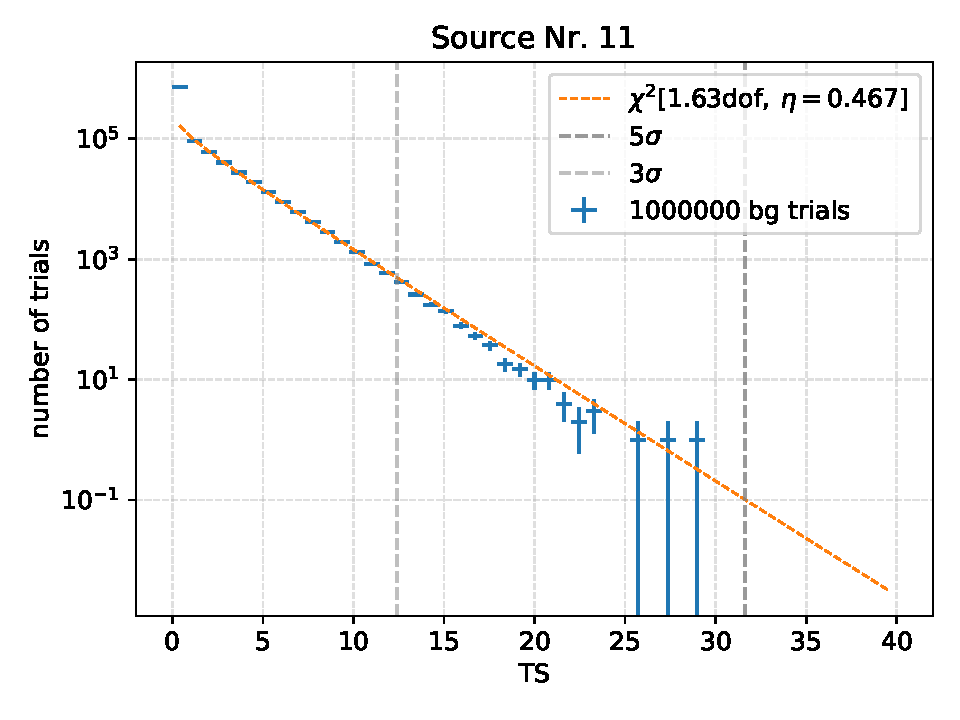
\includegraphics[width=\linewidth]{Plots/05_csky/9_years_gfu_gold_time_dep_bg_t0_1.pdf}
    \caption{Histogram of the background test statistic values for source number $\num{11}$ used in the time-dependent analysis. Shown are also the number of degrees of freedom $dof$ and the ratio of positive and negative values $\eta$. The id of the source corresponds to table \ref{tab:sources} or \ref{tab:sources_time_dep} respectively.}
    \label{fig:bg_trials_time_dep_1}
\end{figure}
\begin{table}
  \centering
  \caption[]{Table of number of trials, degrees of freedom $dof$, symmetry parameter $\eta$, median\footnotemark, $\num{3}\sigma$ and $\num{5}\sigma$ values of the background test statistics for the time-dependent analysis for all $\num{10}$ sources seen in figure \ref{fig:bg_trials_time_dep}.}
  \begin{tabular}{crccccc}
    \toprule
    Nr. & trials & $dof$ & $\eta$ & median & $\num{3}\sigma$ & $\num{5}\sigma$ \\
    \toprule
      11 & 0.000 & 12.413 & 31.600 \\ 12 & 0.000 & 13.171 & 33.390 \\ 13 & 0.079 & 14.013 & 34.950 \\ 16 & 0.030 & 13.735 & 34.461 \\ 29 & 0.000 & 13.471 & 33.910 \\ 37 & 0.000 & 13.436 & 33.919 \\ 42 & 0.000 & 13.642 & 34.476 \\ 43 & 0.005 & 13.395 & 33.752 \\ 58 & 0.000 & 13.587 & 34.041 \\ 63 & 0.000 & 12.909 & 32.821 \\ 
    \toprule
    \label{tab:sigma_time_dep}
  \end{tabular}
\end{table}
\footnotetext{Some median values are very close to if not $\num{0}$.}
\begin{figure}
    \centering
    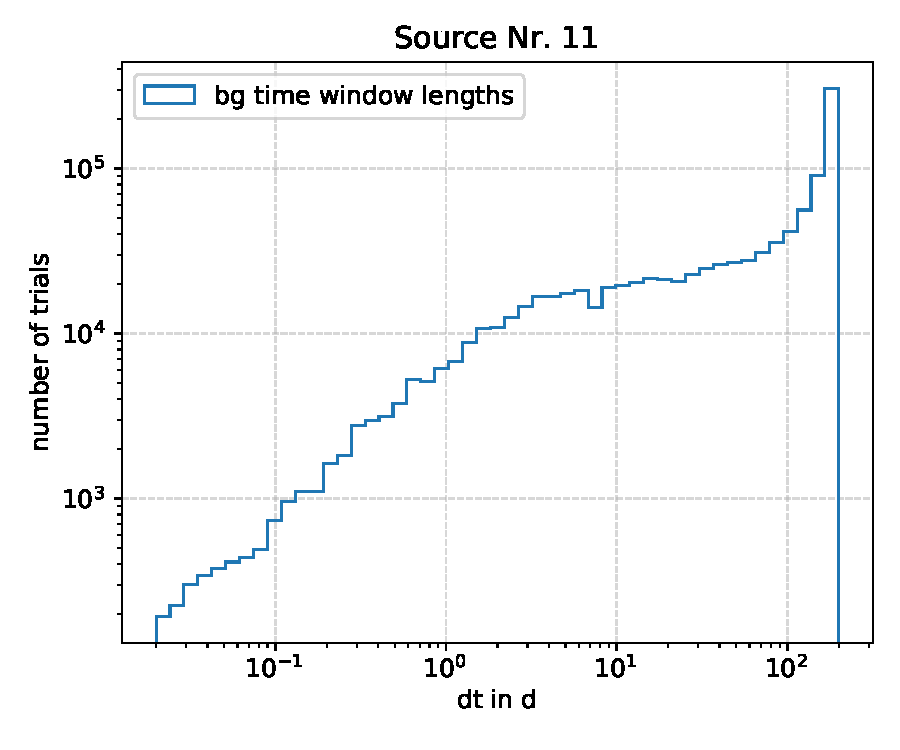
\includegraphics[width=\linewidth]{Plots/05_csky/9_years_gfu_gold_time_dep_bg_dt_1.pdf}
    \caption{Histogram of the background time window lengths $dt$ in days of source number $\num{11}$ for the time-dependent analysis.}
    \label{fig:bg_trials_time_dep_time_windows_1}
\end{figure}
\begin{figure}
    \centering
    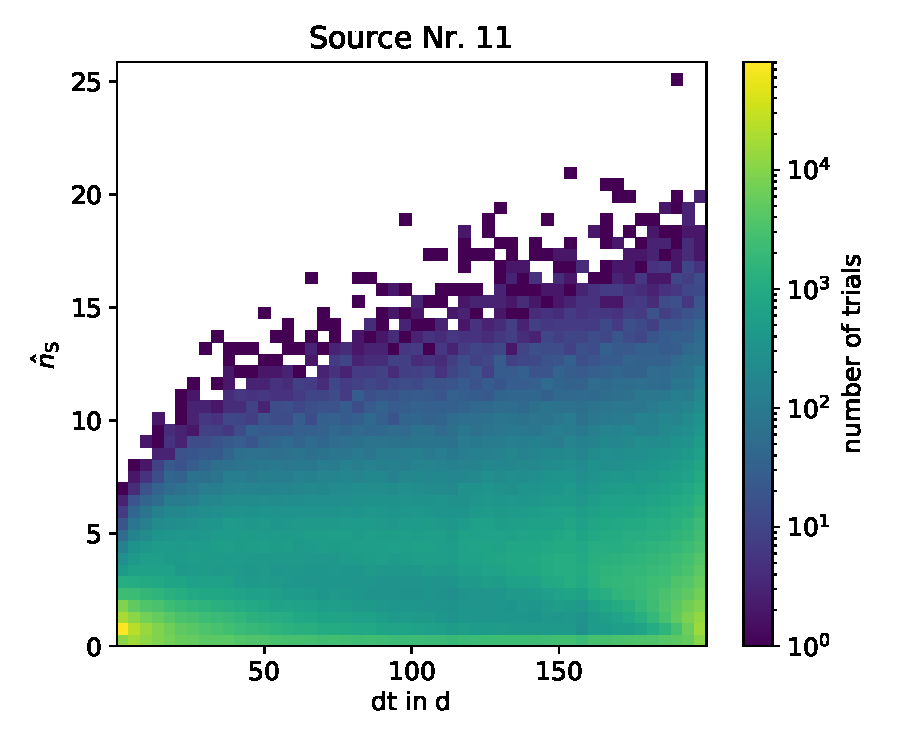
\includegraphics[width=\linewidth]{Plots/05_csky/time_window_ns_bg_time_dep_1.pdf}
    \caption{Histogram of the fitted number of signal events $\hat{n}_\text{S}$ in dependence of the time window lengths $dt$ in days of the background trials for the time-dependent analysis for source number $\num{11}$.}
    \label{fig:bg_trials_time_dep_time_windows_ns_1}
\end{figure}

\section{Signal Trials}

As in the time-integrated analysis, a likelihood scan is first considered to ensure a well-defined maximum and a generally smooth environment, so that a problem with the fit and the set parameters can be excluded.
This scan is shown for source number $\num{11}$ in figure \ref{fig:llh_scan_time_dep} and for all sources in figure \ref{fig:llh_scan_time_dep_all}.
\begin{figure}
    \centering
    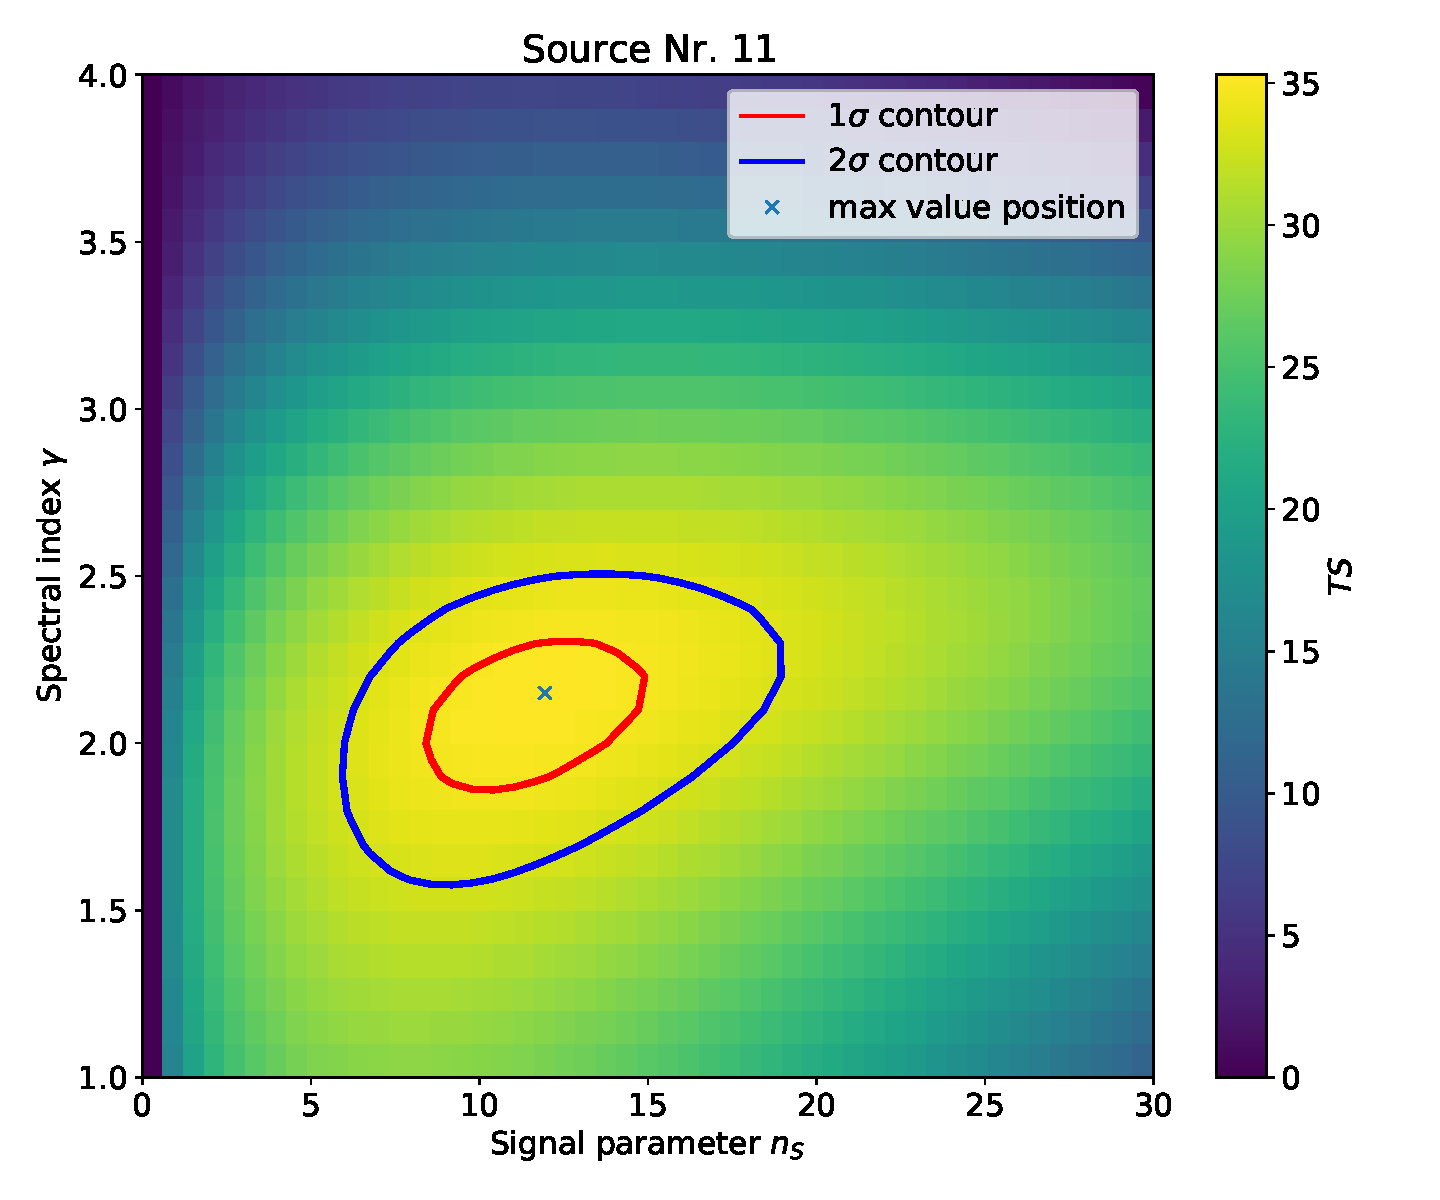
\includegraphics[width=\linewidth]{Plots/05_csky/llh_scan_1.pdf}
    \caption{Scan of the likelihoodspace for source number $\num{11}$ with a timewindow of $\SI{200}{\day}$ for the time-dependent analysis. The scan is in the spectral index $\gamma$ and the signal parameter $n_\text{S}$. The number of induced signal events is $n_S = \num{10}$ with a spectral index of $\gamma = 2$. The maximum test statistic value is marked in the plot including the contours of $\num{1}\sigma$ and $\num{2}\sigma$ and source number corresponds to table \ref{tab:sources}.}
    \label{fig:llh_scan_time_dep}
\end{figure}
After a proper likelihood environment is ensured, the signal trials can be started.
The number of trials per source and the corresponding number of injected signal events can be seen in table \ref{tab:trials_sig_time_dep_table}.
The resulting CDFs in terms of sensitivity and discovery potential are shown in figure \ref{fig:time_dep_cdf_sens_disc_1}.
\begin{figure}
    \centering
    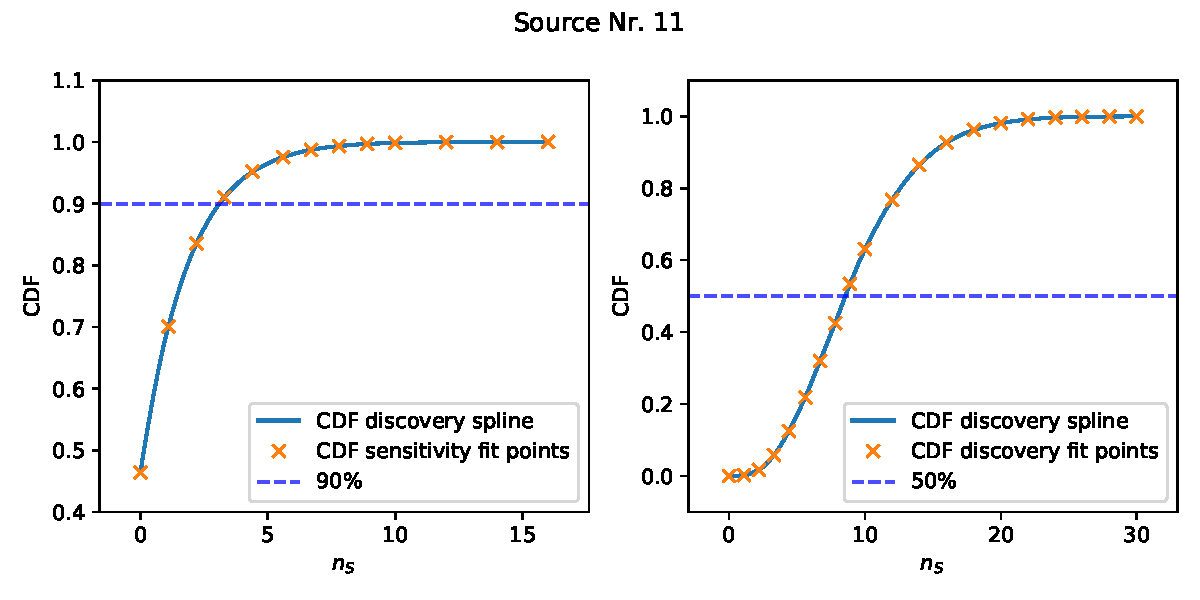
\includegraphics[width=\linewidth]{Plots/05_csky/9_years_gfu_gold_time_dep_cdf_1.pdf}
    \caption{Quantiles of the signal trials for the calculation of the sensitivity for the time-dependent analysis of source number $\num{11}$ on the left and discovery potential on the right at a spectral index of $\gamma=\num{2}$. A $\chi^2$ CDF fit provides a more accurate estimate of the sought signal parameter $n_\text{S}$ which satisfies the condition of the sensitivity at $\SI{90}{\percent}$ and discovery potential at $\SI{50}{\percent}$ respectively, both represented via a dashed line.}
    \label{fig:time_dep_cdf_sens_disc_1}
\end{figure}
From this, the fluences for the sensitivity and the discovery potential can be calculated. These are listed in table \ref{tab:sens_disc_time_dep} for all sources and additionally presented in dependence on their position in the sky in figure \ref{fig:sens_disc_time_dep}.
\begin{figure}
    \centering
    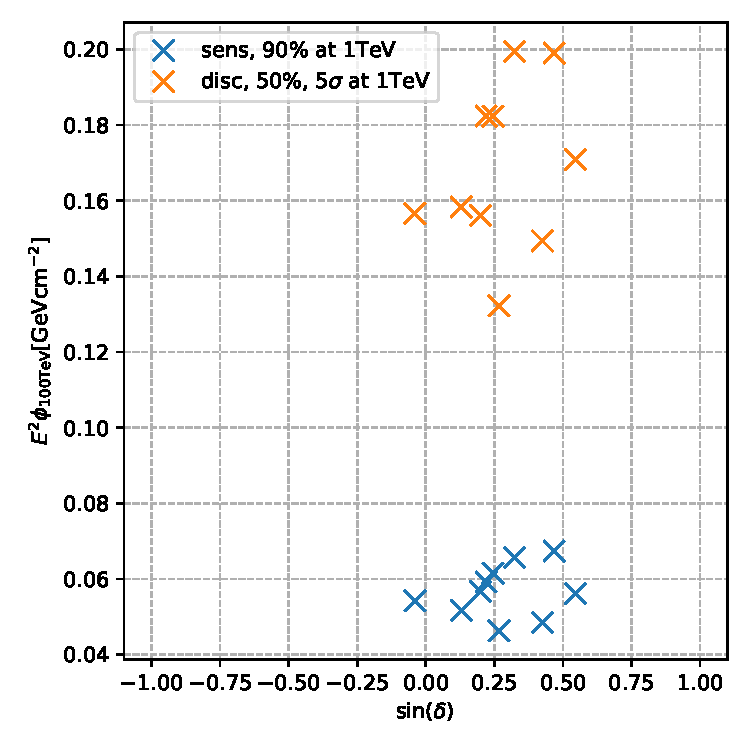
\includegraphics[width=10cm]{Plots/05_csky/time_dep_sens_disc_dec.pdf}
    \caption{Sensitivities and discovery potentials for all $\num{10}$ sources in dependece of their position at a reference energy of $E_0 = \SI{1}{\tera\electronvolt}$ for the time-dependend analysis.}
    \label{fig:sens_disc_time_dep}
\end{figure}
\begin{table}
  \centering
  \caption{Sensitivities and discovery potentials for different sources at a reference energy of $E_0 = \SI{1}{\tera\electronvolt}$ and a spectral index $\gamma=2$ for the time-dependent analysis. Additionally the sine of the source declination $\delta$ and the fitted number of signal events $N_\text{sig}$ satisfying the thresholds is shown.}
  \begin{tabular}{ccrcrc}
    \toprule
    Nr. & $\sin{(\delta)}$ & $N_\text{sig,sens}$ &  sens in $\si{\giga\electronvolt\centi\meter\tothe{-2}}$ & $N_\text{sig,disc}$ & disc in $\si{\giga\electronvolt\centi\meter\tothe{-2}}$ \\
    \toprule
      11 & 0.199 & 3.10 & \num{5.67e-2} & 8.53 & \num{1.56e-1} \\ 12 & 0.245 & 3.04 & \num{6.15e-2} & 9.01 & \num{1.82e-1} \\ 13 & 0.425 & 2.83 & \num{4.85e-2} & 8.71 & \num{1.49e-1} \\ 16 & 0.129 & 2.91 & \num{5.17e-2} & 8.91 & \num{1.58e-1} \\ 29 & 0.220 & 2.87 & \num{5.93e-2} & 8.84 & \num{1.82e-1} \\ 37 & 0.324 & 2.95 & \num{6.57e-2} & 8.94 & \num{1.99e-1} \\ 42 & 0.468 & 2.99 & \num{6.74e-2} & 8.84 & \num{1.99e-1} \\ 43 & 0.545 & 2.97 & \num{5.61e-2} & 9.03 & \num{1.71e-1} \\ 58 & 0.267 & 2.33 & \num{4.63e-2} & 6.65 & \num{1.32e-1} \\ 63 & -0.040 & 3.01 & \num{5.43e-2} & 8.69 & \num{1.57e-1} \\ 
    \toprule
    \label{tab:sens_disc_time_dep}
  \end{tabular}
\end{table}
In addition, as with the background trials, the distribution of the time window lengths can be studied.
Here, the set of signal trials is considered for which the injected signal parameter is closest to the required signal for the satisfaction of the condition for sensitivity and the discovery potential seen in table \ref{tab:sens_disc_time_dep}.
The resulting test statistics are additionally given in the appendix in plots \ref{fig:time_dep_sig_sens_ts} and \ref{fig:time_dep_sig_disc_ts}.
The time window length distributions can be seen in figure \ref{fig:sens_disc_dt_1}.
\begin{figure}
    \centering
    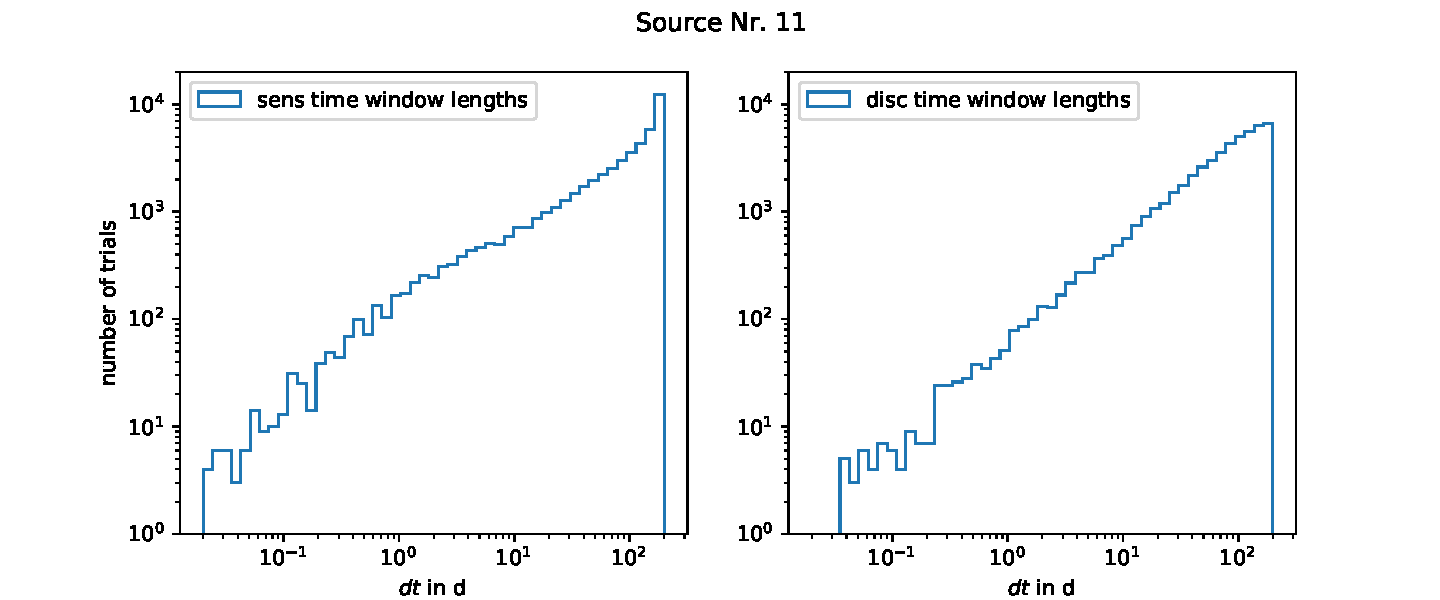
\includegraphics[width=\linewidth]{Plots/05_csky/9_years_gfu_gold_disc_sens_time_dep_dt_1.pdf}
    \caption{Histograms of the time window lengths $dt$ in days of source number $\num{11}$ for the time-dependent analysis for the set of signal trials with the number of injected signal events closest to satisfying the condition to calculate the sensitivity on the left and discovery potential on the right.}
    \label{fig:sens_disc_dt_1}
\end{figure}
It can be seen that more small to medium time windows are possible for the calculation of the sensitivity.
For the calculation of the discovery potential, larger time windows are generally required.
Therefore, the distribution towards the maximum time window length is flatter than for sensitivity.
The fitted signal parameter in dependence of the time window length can be seen in figure \ref{fig:sens_disc_ns_dt_1}.
\begin{figure}
    \centering
    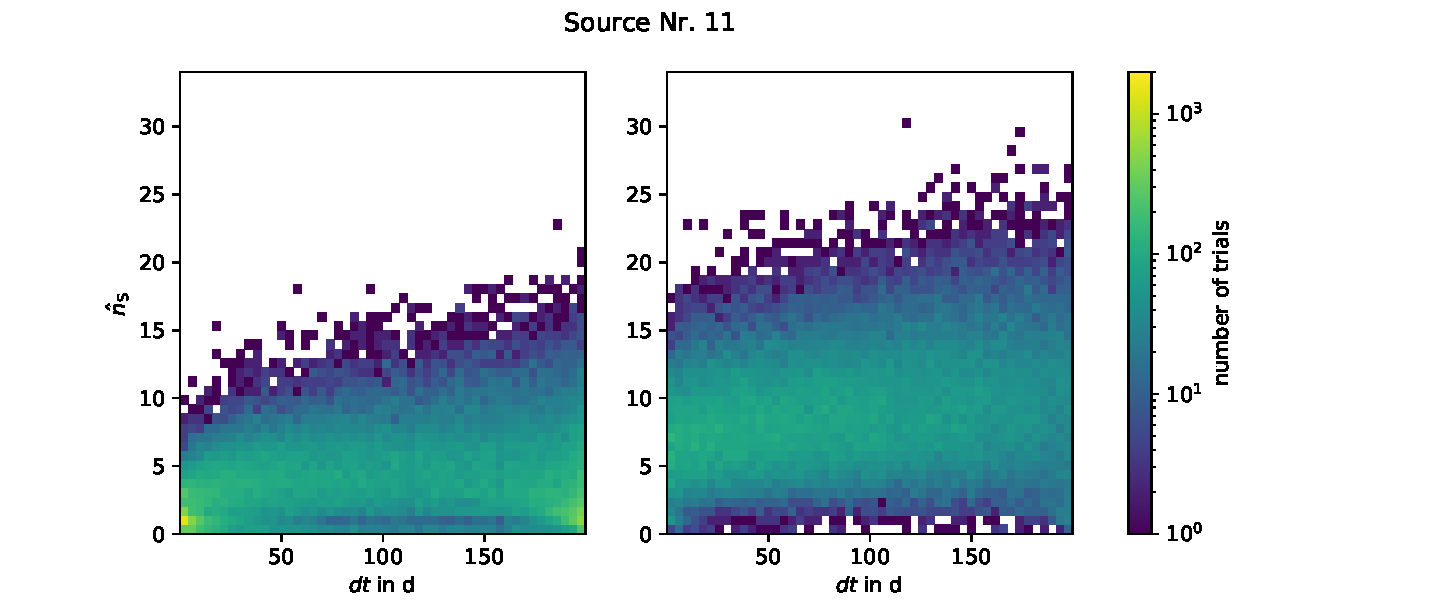
\includegraphics[width=\linewidth]{Plots/05_csky/time_window_ns_disc_sens_time_dep_1.pdf}
    \caption{Histograms of the time window lengths $dt$ in days in dependence of the fitted signal parameter $\hat{n}_\text{S}$ of source number $\num{11}$ for the time-dependent analysis for the set of signal trials with the number of injected signal events closest to satisfying the condition to calculate the sensitivity on the left and discovery potnetial on the right.}
    \label{fig:sens_disc_ns_dt_1}
\end{figure}
As expected, it can be seen that the determination of sensitivity requires less signal than the determination of the discovery potential.
The distribution of sensitivity shows a clear tendency towards smaller signal parameters, whereas the distribution of discovery potential is much broader.
It is interesting to note, however, that for both distributions an arc around signal parameters just above $\hat{n}_\text{S}=0$ can be observed for medium time windows.
Larger time windows allow for more signal, but the fact that the possible signal parameter decreases again towards the maximum length is strange and could have something to do with the combinatorics of the length of the time window and the signal or with the time window fit in general, since signal parameter and the setting of the time window are not independent of each other.

\section{Examination of Fit Bias}

To check the correctness of the fits, the fitted spectral index $\hat\gamma$ and the number of signal events $\hat{n}_\text{S}$ are again checked for bias.
The plots used to examine the fit bias are shown in figure \ref{fig:ns_gamma_fit_time_dep_1} for source number $\num{11}$ and for all sources in the appendix \ref{sec:fit_bias_time_dep}.
Here, as well, the minimum fitted signal parameter $\hat{n}_\text{S}$ is approximately $\num{2}$, since the time windows are expanded between two events.
In the environment of sensitivity and discovery potential ($2 < n_\text{S} < 10$), the signal parameter is somewhat overestimated.
Above this, the fit slowly approaches the true value.
This shifts the final results to higher values, but this only makes the analysis more conservative.
The value for the spectral index starts at $\hat\gamma \approx 3$, as already explained in the previous analysis.
It slowly approaches the true value for a higher number of injected events.
A higher spectral index gives the individual signal events a smaller weight, which means that more signal is required to bring the test statistic values over a certain threshold.
\begin{figure}
    \centering
    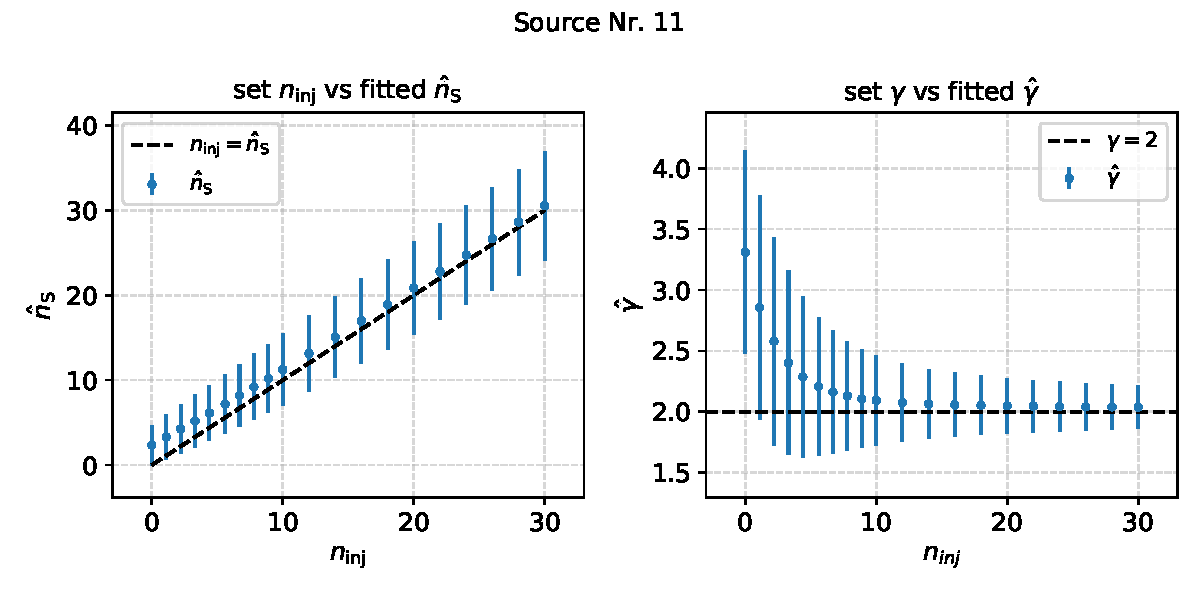
\includegraphics[width=\linewidth]{Plots/05_csky/ns_gamma_fit_time_dep_1.pdf}
    \caption{On the left: Fitted number of signal events $\hat{n}_{\text{S}}$ in dependence of the injected number of signal events $n_\text{inj}$ with spectral index $\gamma = 2$ for the time-dependent analysis. The black dashed line shows the equality of fitted and injected number of signal events. On the right: Fitted spectral index $\hat\gamma$ in dependence of the injected number of signal events $n_\text{inj}$ with spectral index $\gamma = 2$, shown with a horizontal black dashed line, for the trials used in the time-dependent analysis.}
    \label{fig:ns_gamma_fit_time_dep_1}
\end{figure}
